\section{Task 1: Understanding HSRN researchers' needs and behaviors}

\begin{figure}[t]
    \centering
    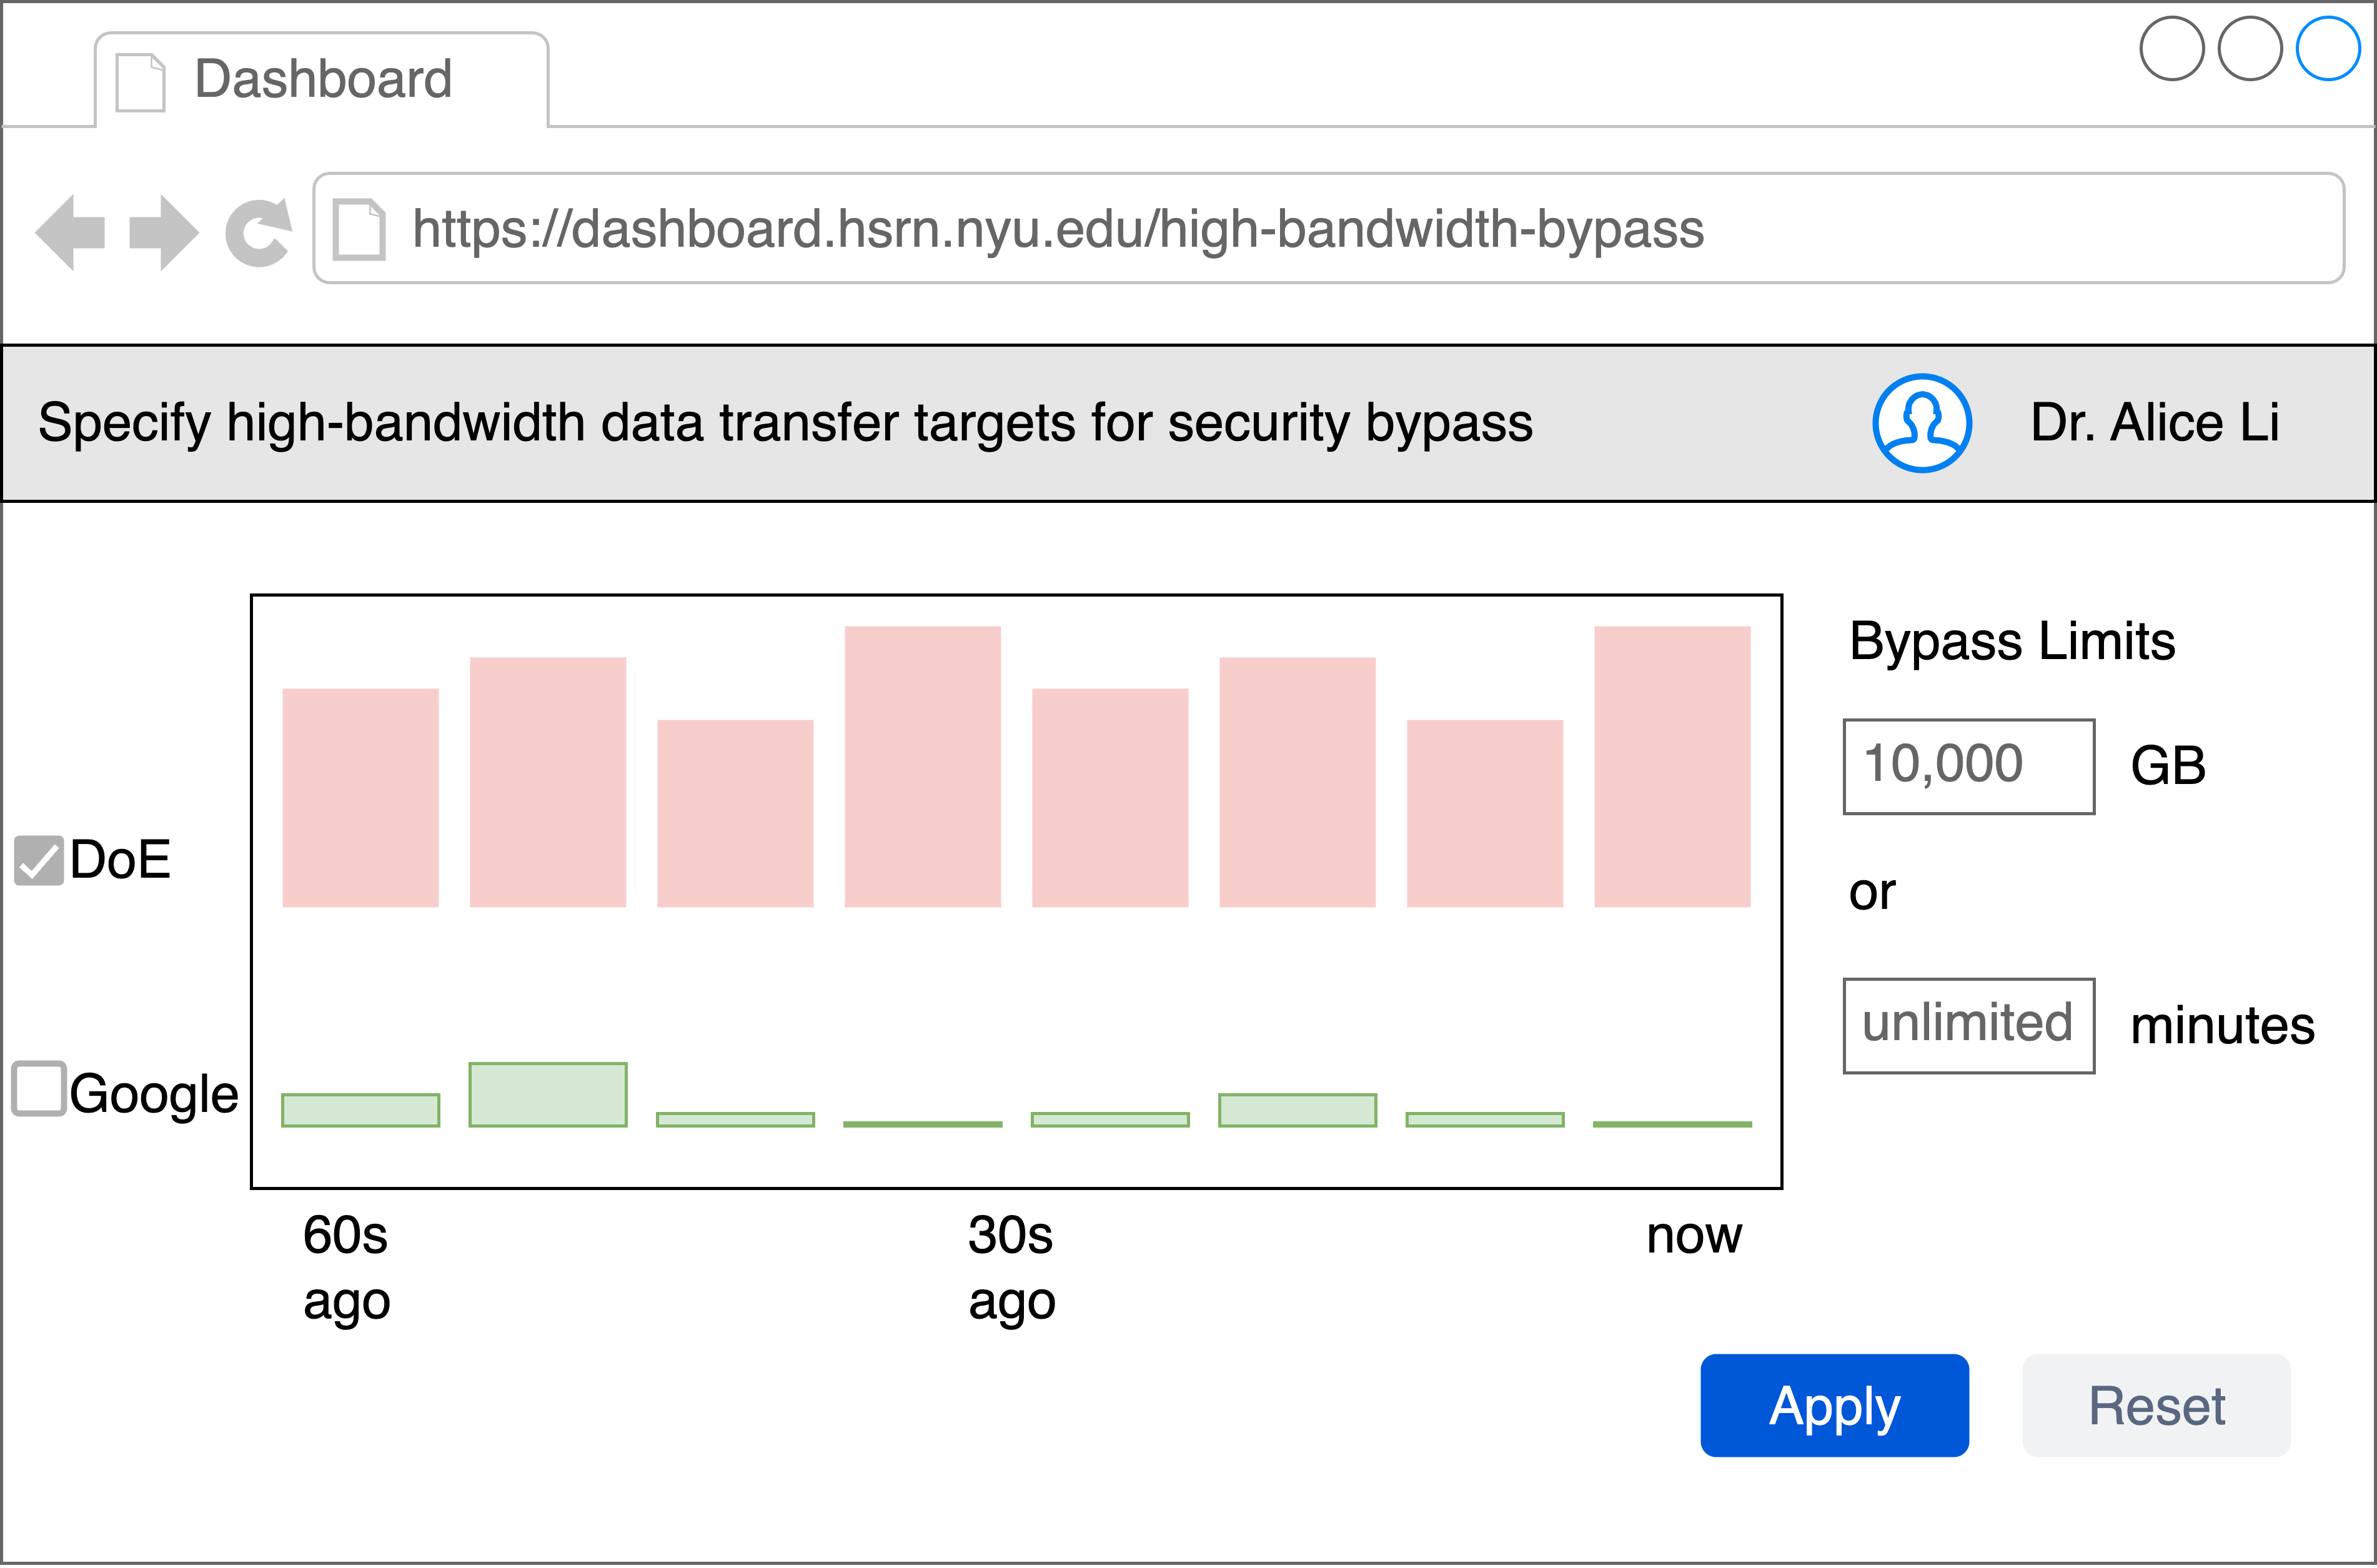
\includegraphics[width=0.7\linewidth]{figures/dashboard.png}
    \caption{A sample of the dashboard's user interface.}
    \label{fig:dashboard}
\end{figure}

Before we implement the system, we first need to understand the needs of researchers as reported by researchers, e.g., how they interact with the current HSRN, how they currently request security bypasses with the network administrators, what are their concerns, and what they would like to see as a solution. This human-centered understanding will help us design the user interface and user experience (UI/UX). We will provide the details in Task 1a.

In addition, we will also need to understand the researchers' behaviors as reported by the network traffic, e.g., their network activities and traffic patterns, by conducting passive network measurements. This analysis will facilitate the automatic annotation of the network traffic of users, e.g., which remote destinations the users are contacting and the estimated bandwidth and latency requirements. Such annotations will help us create the initial allow list, annotate the existing workflow, and help researchers make informed decisions when requesting security bypasses in the UI/UX. We will provide the details in Task 1b.

\subsection{Task 1a: Understanding researchers' needs through user studies}

\paragraph{Understanding existing concerns}
Currently, users on NYU's HSRN would go through a manual approval process to request a temporary bypass for their scientific network traffic, such as sending large datasets or initiating low-latency experiments, e.g., AR/VR. Such requests are often highly technical in nature, including such parameters as the wall ports, remote IP addresses, remote ports, and protocols (TCP/UDP), which, accordingly our preliminary experience with users, could be frustrating for many researchers who do not have the necessary technical background. Furthermore, based on preliminary interviews with network administrators at NYU Research Technologies (where co-PI Pahle is a Senior Research Scientist), this process is also frustrating with network administrators, who often have to manually craft the switch rules based on the researchers' requests. We have also heard of instances where a network administrator had forgotten to disable such a security bypass, thus exposing the researcher to unncessary security risks.

To address these issues, we plan to conduct interviews and focus groups to understand the existing pain points. We will recruit volunteers from within the current users' of NYU HSRN. We will set up 30-minute one-on-one semi-structured interviews with individuals, or 60-minute guided focus groups comprising 3-4 researchers, where we ask them to describe their current experience with NYU's HSRN, e.g., what is their usual scientific workload (such as high-bandwidth transfers versus low-latency experiments), any noticeable degradations in network performance without security bypasses, steps they took to request security bypasses, how often they would need security bypasses, how long before their requests were granted, and how long they would need their security bypass for. Also, we will discuss the details of the requests, including how they described their scientific workload, the bandwidth/latency requirements, the destination party contacted, and particular challenges translating these workloads into bypass requests in a way that can be understood by network administrators. We will tie all these responses to demographics, including what type of researchers they are, from which department, and their level of technical expertise.

This exercise will help us not only understand the needs of researchers but also build a qualitative profile of invididual researchers in terms of their usual scientific workloads: Who from which department tends to send/receive high-bandwidth versus low-latency traffic to particular hosts on the same network or to the Internet, using which switch port and destination ports, over which protocol (TCP/UDP), and typically over how long or how many bytes. This profile will be useful in helping us construct an initial personalized allow list in Task 2.


\paragraph{Co-designing UI/UX}
We plan to conduct co-design sessions to make preliminary designs on the dashboard's UI/UX, making sure that the design is consistent with the researchers' scientific workflows.
Based on our preliminary analysis, typical scientific workloads include two type of flows: high-bandwidth flows (e.g., for file transfers) and low-latency flows (e.g., for robotics and AR/VR experiments).

From the researcher profile we collected from Task 1a, we will separate the researchers into two groups: one group who self-identifies as conducting mostly high-bandwidth transfer (e.g., physicists sending data to government agencies); and one group who self-identifies as requiring low-latency applications (e.g., roboticists and AR/VR researchers). For each group, we will recruit 3-4 volunteers per co-design session. Within each session, we will ask the participatns to imagine having a self-service portal to specify their workloads and request security bypass---for example, how to describe their workload (e.g., in terms of expected time of completion and number of bytes transffered), how to describe the intended destinations (e.g., in terms of names of government agencies, institutions, IP addresses, or domain names), and how security may play a role in their scientific workloads (e.g., sensitive versus non-sensitive information). During this process, we will guide the participants to sketch out desired user interfaces, how one screen flows to another, and expected actions from each screen.  We will also encourage the participants to design the sketches to integrate into their existing scientific process and avoid impeding their research (unlike the current manual process of requesting security bypasses).

We show an example of a dashboard in Figure~\ref{fig:dashboard} for researchers with high-bandwidth workload. A physicist, for instance, could be regularly transferring large datasets with the Department of Energy (DoE). In one sample use case, the physicist would start the data transfer first, which, by default, goes through the slow path and subject to packet inspection by security appliances. The physicist would now open the dashboard, which lists the bandwidth consumption on his device to various destinations, including DoE and other web traffic (e.g., to Google). We would highlight the DoE transfer because the transfer is already consuming significant bandwidth and also based on user studies the researcher claims their typical workloads include DoE data transfers. This highlight would nudge the researcher toward selecting the DoE network flows for security bypass. Once the physicist clicks the ``Apply'' button, we would expect the system to automatically reroute the ongoing DoE transfer to the fast path (Task 2).


\paragraph{Preliminary work}
We have done some preliminary informal interviews with existing researchers of NYU's HSRN, including roboticists, physicists, AR/VR researchers, and media/arts researchers (whose Letters of Support have been included in this proposal). These informal interviews have revealed much frustration from the researchers in requesting security bypass. Also, we have learned about the two basic types of workloads---i.e., high bandwidth transfers and low latency applications---common across the researchers. These preliminary findings have inspired the initial design of the UI/UX (Figure~\ref{fig:dashboard}) and the overall architecture of the system (Figure~\ref{fig:system}).

Although we have not conducted formal user studies on the UI/UX for this work, past research by PI Huang includes visualizing network flows for non-technical users [CITE Inspector and CHI paper]. For his past work, for instance, PI Huang also conducted extensive interviews and co-design sessions to understand various special needs of network users (in which case the context is smart home networks). To address these needs, PI Huang developed UI/UX that, for instance, included special annotations (similar to Task 2) and highlights (e.g., the DoE highlight in Figure~\ref{fig:dashboard}) to help non-technical users understand the activities on the network. The techniques and lessons are likely transferrable to this proposal.

\paragraph{Expected outcome} We will gain a qualitative understanding of which type of researchers in what departments typically send/receive what kinds of workfloads (i.e., high bandwidth vs low latency); their concerns in the current security bypass process; and their proposed UI/UX for a self-service security bypass tailored to individual needs.



\paragraph{Lead investigator}
PI Huang will lead the user study, assisted by co-PI Pahle, who can help recruit volunteer users of NYU's HSRN into the user study. PI Huang has extensive experience conducting human-centered research.










\subsection{Task 1b: Identifying traffic patterns through network measurement}

While Task 1a provides us with a qualitative understanding of the researchers' needs and behaviors, this data is limited, because they are based on self-reports (therefore subject to biases or errors) and lack a quantitative perspective that would help us design the UI/UX of the dashboard.
This quantitative perspective is important for us to identify scientific workloads (e.g., the high-bandwidth transfers and low-latency applications) versus non-scientific workloads (e.g., typical web traffic); distinguish types of scientific workloads (e.g., high bandwidth versus low latency); and pinpoint the destination party being contacted in the network flows (e.g., DoE that receives the high-bandwidth data transfer, or the Internet-connected robotic device in the case of low-latency applications).

All of these are critical in helping us create automated annotations to guide users (Task 1b) and identify potential errors (Task 2). Figure~\ref{fig:dashboard} shows an example of traffic annotations. Here, research workloads are shown in red, whereas non-research workloads in green. For each type of workload, the destination parties are annotated to indicate who is interacting with the researcher, along with how many bytes are sent. In this example, the network flows to the Department of Energy (in the case of this hypothetical physicist) is annotated as ``DoE'', while the web traffic is identified as going toward ``Google.'' Such annotations will likely encourage the researcher to select the correct destination---i.e., ``DoE''---on which to apply the security bypass.

We plan to make these annotations by analyzing the existing network traffic of NYU's HSRN users. Co-PI Pahle already has access to a tool called NetBox to visualize the network traffic of the HSRN users. Building on top of this preliminary work, we will mirror existing traffic---by setting up port mirroring, for instance at [B], to a server running Zeek [G], as illustrated in Figure~\ref{fig:system}. We will analyze the Zeek logs to create the following annotations.

\paragraph{Annotating research workloads and destinations}
We plan to identify research versus non-research workloads based on the destination contacted. However, even to make annotations such as ``user contacting DoE servers'' or ``user contacting Google services'' is not trivial. There are two main challenges for identifying  destinations.

The first challenge is inferring the hostnames.


\paragraph{Annotating types of research workloads}
high bandwidth vs low latency

In task one be our goal is to basically come up with default configurations for the allowed lists. At the end of the day, these researchers, we need to help them Bootstrap. Basically, when they first open the dashboard, the dashboard shows some default settings that already fit their needs.

For example, if this is a physicist who regularly sends large amounts of data to say, the Department of Energy, the dashboard should come with pre configured settings for enabling transfers to Department of Energy. So we come up with these default values from two sources. One is from task one a where we find out you know, what the usual regular workflows from the visa researchers are based on their self reports. And based on, you know, this quality of qualitative data. That's the first source.

We need to help researchers make a decision. Bootstrap the allow list. Initial annotations.



\paragraph{Clustering scientific workloads}
Understand qualitatively what kind of network traffic they send. Elephant flows, or latency sensitive flows, presumably depending on what kind of experiment or research work they do.


cluster scientific traffic (based on the surveys and interviews): elephant flows (applicants that consumer significant bandwidth), or flows with small, consistent inter-arrival times (latency sensitive applications); and cluster users: AR researchers vs chemistry researchers who send data to DoE




The second source would be coming from network measurement data. We can look at these researchers network traffic. For example, for this physicist, we were able to identify things like this researcher does indeed send a large number of bytes to a server with a domain name that ends with do E and or the autonomous system number belongs to a D O E Network.

This not only helps us This not only helps us confirm the user self report, but it also provides us with a set of quantitative metrics for just identifying the workflows, for example, the workflows will be in the form the the end of it is for a way for us to create annotations of their workflows for example, in this case, the work the annotation would be source coming from this researcher and destination going to particular IP address or the DNS would correspond to a doe domain.

We will learn this data from several sources one from existing data collection mechanisms In a case of NYU, we have this thing called a net box that has analyzed data. Another way we propose is that we will stick this Zeke box into the network, which captures network traffic through a, a tap port, which mirrors the traffic, who is Zeke instance. And that would record basically what DNS traffic is captured. And also, what's the destination IP addresses. And various flow statistics like the total number of bytes, the duration of flows, and, you know, things like inter packet arrival times, which is important in characterizing low latency applications.

So, basically, in summary, the second task, I'm sorry, task one B will help us generate a set of annotations for network traffic, that would quantitatively describe various workflows for these researchers, workflows, that are high bandwidth in nature, or workflows that are low latency in nature for different kinds of researchers. So that's task one, B.





Clustering flows. Based on Task 1a, we know qualitatively what kinds of flows researchers tend to generate. Can we identify them? Can we cluster their network activities on the network and match against the qualitative study? For a data transfer, is it mostly elephant flows to a single destination vs mice flows?


\paragraph{Identifying destinations}
What about destinations? Let's say transfer to DoE — is it just one server, or multiple? External vs internal destinations?

\paragraph{Preliminary work} We spoke to some of the users about their work flows

// netbox already captures who is on which port and use case; flows to help us troubleshoot network speed.

no ipv6; too much work




On the dashboard users need to specify which of their network activities to add to an allow list. Not an easy process. Many flows on their computers, elephant and mice. Also multiple destinations, sometimes to CDNs. We help them make this decision.

Profiling users. Task 1a and 1b already give us user profiles.

Auto-identifying destinations. What destination are you talking to? Not straightforward. PI Huang has some preliminary work. NLP. Zeek logs

Auto-clustering traffic patterns. Identifying elephant flows and latency sensitive flows. Presenting this information through dashboard.  Zeek.

// Idea: identifying network flows

\paragraph{Preliminary work} Inspector work — identifying hosts, based on webXray. Flow clustering: PI Huang's HotSDN paper.

\paragraph{Expected outcome} A technique to automatically identify destinations and traffic patterns to help users make decisions more easily.

\paragraph{Lead investigator} PI Huang and Co-PI Pahle will work together on implementing. Co-PI Cappos will advise on XXX.



\paragraph{Expected outcome} A measurement analysis. Clusters per researcher and type of researcher.

\paragraph{Lead investigator} Co-PI Pahle will work with IT to conduct the study, as he's already a part of the NYU research IT infrastructure team. PI Huang to help with the anonymized data analysis. PI Huang is familiar with network measurement and big data analytics.
